
\documentclass[12pt,openright,oneside,a4paper,english,french,spanish,brazil]{abntex2}

\usepackage{cmap}	
\usepackage{lmodern}	
\usepackage[T1]{fontenc}	
\usepackage[utf8]{inputenc}		
\usepackage{lastpage}		
\usepackage{indentfirst}
\usepackage{color}	
\usepackage{graphicx}	
\usepackage{units}
\usepackage[brazilian,hyperpageref]{backref}
\usepackage[alf]{abntex2cite}
\usepackage{bold-extra}
\usepackage{eso-pic}
\usepackage{nomencl}
\usepackage{tabularx}
\usepackage{pdfpages}
\usepackage{float}
\usepackage{trivfloat}
\usepackage{newfloat}
\renewcommand{\backrefpagesname}{Citado na(s) página(s):~}
\renewcommand{\backref}{}
\renewcommand*{\backrefalt}[4]{
	\ifcase #1 %
		Nenhuma citação no texto.%
	\or
		Citado na página #2.%
	\else
		Citado #1 vezes nas páginas #2.%
	\fi}%
% ---

\DeclareFloatingEnvironment[fileext=lop,
listname={Lista de quadros},placement={!ht},name=Quadro]{quadro}

\counterwithout{quadro}{chapter}

\usepackage{fixos/customizacoes}
\usepackage{multirow}
\usepackage{url}
\usepackage{tabularx}
\usepackage{graphicx} 
\usepackage{ifthen}
\usepackage{amssymb}
\usepackage{adjustbox}   
\usepackage{emptypage}
\newboolean{showcomments}
\setboolean{showcomments}{true}

\ifthenelse{\boolean{showcomments}}
  {\newcommand{\nb}[2]{
    \fcolorbox{gray}{yellow}{\bfseries\sffamily\scriptsize#1}
    {\sf\small$\blacktriangleright$\textit{#2}$\blacktriangleleft$}
   }
   \newcommand{\version}{\emph{\scriptsize$-$working$-$}}
  }
  {\newcommand{\nb}[2]{}
   \newcommand{\version}{}
  }

\newcommand\info[1]{\nb{Info}{#1}}
\newcommand\todo[1]{\nb{ToDo}{#1}}


\newcommand\carla[1]{\nb{Carla}{#1}}
\newcommand\Carla[1]{\nb{Carla}{#1}}


% Dados pessoais
    \autor{Caio César Oliveira}
\curso{Engenharia de Software}

% Dados do trabalho
\titulo{Desenvolvimento de uma Inteligência Artificial para Aprimoramento da Avaliação Individual em Disciplinas de Software na Universidade de Brasília}
\data{2024}
\palavraChaveUm{Construção}
\palavraChaveDois{feedback}
\palavraChaveTres{relevante}

% Dados da orientacao
\orientador{Prof. Dr. George Marsicano}

% Dados para a ficha catalográfica
\cdu{02:141:005.6}

% Dados da aprovação do trabalho
\dataDaAprovacao{x de y de 202z}
\membroConvidadoUm{}
\membroConvidadoDois{}
\membroConvidadoTres{}

\local{Brasília, DF}
\instituicao{%
  Universidade de Brasília -- UnB
  \par
  Faculdade UnB Gama -- FGA
}
\tipotrabalho{Trabalho de Conclusão de Curso}
\preambulo{Monografia submetida ao curso de graduação em \imprimircurso\ 
da Universidade de Brasília, como requisito parcial para obtenção do Título 
de Bacharel em \imprimircurso.}

\definecolor{blue}{RGB}{41,5,195}
\makeatletter
\hypersetup{
     	%pagebackref=true,
		pdftitle={\@title}, 
		pdfauthor={\@author},
    	pdfsubject={\imprimirpreambulo},
	    pdfcreator={LaTeX with abnTeX2},
		pdfkeywords={abnt}{latex}{abntex}{abntex2}{trabalho acadêmico}, 
		colorlinks=true,       		% false: boxed links; true: colored links
    	linkcolor=blue,          	% color of internal links
    	citecolor=blue,        		% color of links to bibliography
    	filecolor=magenta,      		% color of file links
		urlcolor=blue,
		bookmarksdepth=4
}
\makeatother
\setlength{\parindent}{1.3cm}
\setlength{\parskip}{0.2cm}  
\makeindex



\begin{document}

\frenchspacing 
\imprimircapa
\imprimirfolhaderosto*

\begin{fichacatalografica}
	\vspace*{\fill}					% Posição vertical
	\hrule							% Linha horizontal
	\begin{center}					% Minipage Centralizado
	\begin{minipage}[c]{12.5cm}		% Largura
	
	\imprimirautor
	
	\hspace{0.5cm} \imprimirtitulo  / \imprimirautor. --
	\imprimirlocal, \imprimirdata-
	
	\hspace{0.5cm} \pageref{LastPage} p. : il. (algumas color.) ; 30 cm.\\
	
	\hspace{0.5cm} \imprimirorientadorRotulo~\imprimirorientador\\
	
	\hspace{0.5cm}
	\parbox[t]{\textwidth}{\imprimirtipotrabalho~--~\imprimirinstituicao,
	\imprimirdata.}\\
	
	\hspace{0.5cm}
		1. \imprimirpalavrachaveum.
		2. \imprimirpalavrachavedois.
		3. \imprimirpalavrachavetres.
		I. \imprimirorientador.
		II. Universidade de Brasília.
		III. Faculdade UnB Gama.
		IV. \imprimirtitulo\\ 			
	
	\hspace{8.75cm} CDU \nomecdu\\
	
	\end{minipage}
	\end{center}
	\hrule
\end{fichacatalografica}
\clearpage


\begin{folhadeaprovacao}

  \begin{center}
    {\ABNTEXchapterfont\large\imprimirautor}

    \vspace*{\fill}\vspace*{\fill}
    {\ABNTEXchapterfont\bfseries\Large\imprimirtitulo}
    \vspace*{\fill}
    
    \hspace{.45\textwidth}
    \begin{minipage}{.5\textwidth}
        \imprimirpreambulo
    \end{minipage}%
    \vspace*{\fill}
   \end{center}
    
   Trabalho aprovado. \imprimirlocal, \imprimirdatadaaprovacao:

   \assinatura{\textbf{\imprimirorientador} \\ Orientador} 
   \assinatura{\textbf{\imprimirmembroconvidadoum} \\ Convidado 1}
   \assinatura{\textbf{\imprimirmembroconvidadodois} \\ Convidado 2}
   \assinatura{\textbf{\imprimirmembroconvidadotres} \\ Convidado 3}
      
   \begin{center}
    \vspace*{0.5cm}
    {\large\imprimirlocal}
    \par
    {\large\imprimirdata}
    \vspace*{1cm}
  \end{center}
  
\end{folhadeaprovacao}

\begin{agradecimentos}

\subsection*{Caio César Oliveira}

Gostaria de expressar meu mais profundo agradecimento a Deus, cuja graça e orientação têm sido fundamentais em minha jornada. Também não posso deixar de agradecer meus amados pais, Rozana Maria de Oliveira e Fábio Batista Oliveira, por seu apoio inabalável, encorajamento constante e amor incondicional. Suas palavras de sabedoria e exemplo de dedicação têm sido uma fonte de inspiração para mim. 
Além disso, desejo expressar minha gratidão à minha amada namorada, Nicole Soares dos Santos, que tem sido meu porto seguro, meu apoio emocional e minha maior incentivadora. Suas presenças na minha vida têm sido um verdadeiro presente, trazendo alegria e motivação em todos os momentos.
Uma gratidão especial à Universidade de Brasília, as experiências adquiridas ao longo do curso de Engenharia de Software foram enriquecedoras e fundamentais para o meu crescimento pessoal, acadêmico e profissional. Agradeço a todos os professores, colegas e funcionários que contribuíram para o meu aprendizado e desenvolvimento, a todo o corpo docente, que possui toda uma estrutura de qualidade para uma boa educação.
Por fim, agradeço  meu orientador, o doutor George Marsicano Corrêa, por toda sua disponibilidade, dedicação, orientação sábia e conselhos valiosos, que foram cruciais para o desenvolvimento deste trabalho de conclusão de curso.

\end{agradecimentos}

\begin{resumo}

    Esse trabalho se refere ao ambiente educacional da Universidade de Brasília, nas disciplinas requisitos de software e métodos de desenvolvimento de software, onde são realizadas avaliações individuais dessas matérias, utilizando a plataforma Microsoft Forms. 

    O objetivo desse trabalho é desenvolver uma Inteligência Artificial (IA) capaz de aprimorar as avaliações individuais das disciplinas, permitindo que os alunos compreendam seus erros e saibam como evoluir em futuras avaliações por meio de \textit{feedbacks} formativos.

    Para atingir os objetivos delineados, foi implementada uma metodologia de pesquisa mista, incorporando elementos quantitativos e qualitativos. Além disso, para o desenvolvimento da IA foi utilizada a metodologia de desenvolvimento de software Kanban.

    Por fim, como resultado, uma ferramenta de IA, capaz de analisar as informações das respostas dos questionários de avaliação individual dos estudantes (realizados na plataforma Microsoft Forms), e gerar \textit{feedbacks} formativos.

 \vspace{\onelineskip}
    
 \noindent
 \textbf{Palavras-chave}: \textit{Feedback}. qualitativos. quantitativos. Inteligência Artificial. questionários. 
\end{resumo}

\begin{resumo}[Abstract]
 \begin{otherlanguage*}{english}
   This work revolves around the educational environment at the University of Brasília, specifically focusing on the disciplines of Software Requirements and Software Development Methods, where individual assessments are conducted using the Microsoft Forms platform.

    The aim of this study is to develop an Artificial Intelligence system capable of enhancing individual assessments in these disciplines, enabling students to comprehend their mistakes and understand how to evolve in future assessments through formative feedback.

    To achieve the outlined objectives, a mixed research methodology was implemented, incorporating quantitative and qualitative elements. Furthermore, Kanban and Scrum software development methodologies will be used for the development of AI.

    Finally, the result is expected to be an AI tool, capable of analyzing information from the responses of students' individual assessment questionnaires (carried out on the Microsoft Forms platform), and generating formative feedbacks.
   \vspace{\onelineskip}
 
   \noindent 
   \textbf{Key-words}: Feedback. qualitative. quantitative. Artificial Intelligence. tests. 
 \end{otherlanguage*}
\end{resumo}

\pdfbookmark[0]{\listfigurename}{lof}
\listoffigures*
\clearpage
\pdfbookmark[0]{\listtablename}{lot}
\listoftables*

\begin{siglas}
  \item[REQ] Requisitos de Software
  \item[MDS] Métodos de Desenvolvimento de Software
  \item[IA] Inteligência Artificial
  \item[NLP] Processamento de Linguagem Natural
  \item[UnB] Universidade de Brasília
  \item[TCC1] Trabalho de Conclusão de Curso 1
  \item[TCC2] Trabalho de Conclusão de Curso 2

\end{siglas}

\pdfbookmark[0]{\contentsname}{toc}
\tableofcontents*
\cleardoublepage


\textual

\chapter[Introdução]{Introdução}

\section{Contexto}

No âmbito educacional da Universidade de Brasília, questionários aplicados nas disciplinas requisitos de software e métodos de desenvolvimento de software serão administrados através da plataforma Microsoft Forms. Serão aplicados regularmente ao longo do semestre e mensuram o desempenho dos discentes por meio de resultados quantitativos, ou seja, escalas numéricas, além de apresentar a quantidade de respostas certas e erradas visando avaliar o conhecimento dos alunos. 

\section{Problema}

Frequentemente os estudantes enfrentam dificuldades ao receberem resultados de avaliações que utilizam apenas classificações numéricas, pois essas designações, por si só, não fornecem uma compreensão clara do desempenho ou das áreas a serem aperfeiçoadas. Essas mensurações, embora forneçam uma noção geral, não oferecem informações específicas sobre os erros cometidos ou os tópicos que o estudante precisa revisar e consolidar. Isso pode resultar em frustrações e desafios para o estudante, por não entender claramente o resultado de uma avaliação. 

Portanto, o resultado das avaliações individuais apresentadas nas disciplinas requisitos de software e métodos de desenvolvimento de software é apenas quantitativo, uma solução limitada para os estudantes, uma vez que dá ênfase a um \textit{feedback} voltado para avaliações positivas ou negativas do que para um formato formativo. O qual poderia contribuir mais significativamente para a formação do discente e seu desenvolvimento dentro das matérias especificadas.

\section{Justificativa}

O presente trabalho beneficiará diretamente os estudantes ao oferecer \textit{feedbacks} formativos, os quais proporcionam uma análise aprofundada e construtiva do desempenho individual, orientando de maneira mais eficaz para o aprimoramento contínuo. Além disso, os professores e a instituição de ensino também se beneficiarão, podendo aprimorar suas práticas pedagógicas com base nos pontos levantados nos \textit{feedbacks}.

A literatura educacional enfatiza a importância de avaliações detalhadas e direcionadas para um \textit{feedback} formativo, visando promover uma aprendizagem significativa. As discussões no artigo "The Power of Feedback" de Hattie e Timperley \cite{hattie2007}, ressaltam a importância crucial do \textit{feedback} como um elemento fundamental no processo educacional ao apontar seu impacto significativo no desempenho dos alunos, conforme evidenciado por Hattie \cite{hattie2007}. Esse autor realizou uma síntese abrangente de mais de 500 meta-análises, envolvendo um impressionante contingente de 20 a 30 milhões de estudantes, elucidando o impacto substancial que o \textit{feedback} exerce sobre o progresso acadêmico. 

\section{Objetivos}

O objetivo geral do trabalho  é aprimorar o processo de avaliação acadêmica, no que diz respeito as avaliações individuais das disciplinas, requisitos de software e métodos de desenvolvimento de software, utilizando inteligência artificial para construir \textit{feedbacks} formativos individualizados com base no desempenho dos estudantes.

Os objetivos específicos são:

\begin{enumerate}
  \item Identificar as necessidades existentes no atual processo avaliativo individual de estudantes nas disciplinas de requisitos de software e métodos de desenvolvimento de software, em relação aos \textit{feedbacks} recebidos.
  \item Avaliar quais são as necessidades mais relevantes para os discentes.
  \item Desenvolver uma ferramenta utilizando inteligência artificial que seja capaz de analisar o desempenho dos discentes e gerar \textit{feedbacks} formativos personalizados para cada aluno conforme as necessidades levantadas.
  \item Complementar o processo avaliativo individual dos estudantes com \textit{feedbacks} formativos gerados por essa ferramenta, visando aprimorar seu progresso e aprendizado nessas disciplinas.
\end{enumerate}

O objetivo 3, se alinha ao Capítulo 6, o qual analisa a viabilidade técnica do desenvolvimento de uma Inteligência Artificial para aprimorar a avaliação individual nas disciplinas de requisitos de software e métodos de desenvolvimento de software na Universidade de Brasília. Este capítulo explora as tecnologias e ferramentas necessárias para analisar o desempenho dos alunos e fornecer \textit{feedbacks} formativos.

\section{Metodologias}

\begin{table}[!ht]
    \centering
    \begin{tabularx}{\textwidth}{|X|X|X|}
    \hline
        Fase do Trabalho & Objetivos Específicos & Métodos e Técnicas \\ \hline
        \multicolumn{1}{c|}{\multirow{12}{*}{TCC 1}} & Identificar percepções, sentimentos, atitudes
        e idéias dos participantes a respeito de um determinado assunto, produto ou atividade & Grupo Focal \\ \cline{2-3}
        & Coletar dados sobre características, comportamentos ou opiniões de um grupo específico & Survey \\ \cline{2-3}
        & Encontrar materiais relevantes sobre as metodologias utilizadas & Snowballing \\ \cline{2-3}
        & Melhorar a eficiência, qualidade e fluxo de trabalho & Kanban \\ \cline{2-3}
        & Medir a consistência interna dos itens do questionário & Alfa de Cronbach \\ \hline
    \end{tabularx}
    \caption{Tabela de objetivos e técnicas referentes ao TCC 1}
\end{table}


O estudo combina elementos qualitativos e quantitativos para alcançar uma compreensão abrangente do processo avaliativo acadêmico na Universidade de Brasília. A coleta de dados será realizada por meio de análise de resultados em formulários e entrevistas em grupos focais. Os participantes serão estudantes das disciplinas de requisitos de \textit{software} e métodos de desenvolvimento de \textit{software}, que serão selecionados com base em critérios predefinidos para garantir uma representação diversificada e relevante para os objetivos da pesquisa.

As entrevistas em grupos focais com os discentes, permitirão uma compreensão mais aprofundada das percepções dos estudantes, acerca dos desafios enfrentados, ao receberem resultados rasos sobre os questionários realizados. Além disso, serão uma fonte valiosa de \textit{insights} sobre suas sugestões para aperfeiçoar os feedbacks recebidos.

Essa abordagem mista, combinando pesquisa \textit{survey} e entrevistas em grupos focais de discentes nas disciplinas de requisitos de software e métodos de desenvolvimento de software, será essencial para obter uma visão holística das dificuldades enfrentadas pelos estudantes. Os dados coletados fornecerão uma base sólida para aprimorar o processo de avaliação, possibilitando a implementação da Inteligência Artificial, para oferecer feedbacks mais personalizados e eficazes.

\section{Estrutura do Trabalho}

Este trabalho está organizado em uma estrutura que visa oferecer uma análise detalhada e progressiva sobre o tema proposto. A seguir, são apresentados os principais capítulos que compõem esta pesquisa:

\begin{itemize}
    \item \textbf{Capítulo 1 - Introdução}: Apresenta uma visão geral do tema, os objetivos da pesquisa, a justificativa e a metodologia adotada.
    
    \item \textbf{Capítulo 2 - Referencial Teórico}: Constrói as bases teóricas do estudo, abrangendo desde conceitos fundamentais até modelos e teorias relacionadas ao tema específico.
    
    \item \textbf{Capítulo 3 - Metodologias}: Detalha o design da pesquisa, métodos e submétodos escolhidos, explicando a coleta e análise de dados.
    
    \item \textbf{Capítulo 4 - Execução da Pesquisa e Resultados}: Apresenta o processo de execução da pesquisa, incluindo cronograma e etapas do estudo, além da exposição dos resultados brutos.
    
    \item \textbf{Capítulo 5 - Análise dos Resultados}: Interpreta os resultados brutos, transformando-os em percepções e discutindo-os em relação aos objetivos e hipóteses do estudo.
    
    \item \textbf{Capítulo 6 - Análise de Viabilidade Técnica}: Enfoca a viabilidade prática da aplicação baseada em inteligência artificial para promover \textit{feedbacks} formativos, abordando objetivos técnicos, requisitos da ferramenta e tecnologias idealizadas.
    
    \item \textbf{Capítulo 7 - Planejamento}: Apresenta o planejamento das atividades realizado no primeiro período do trabalho, e o planejamento previsto para o segundo período.

    \item \textbf{Capítulo 8 - Considerações Finais da Pesquisa}: Apresenta um resumo das descobertas, implicações, sugestões para estudos futuros e a conclusão do trabalho de pesquisa.

    \item \textbf{Capítulo 9 - Desenvolvimento da Ferramenta de Feedback Formativo - FeedFor}: Apresenta um aglomerado de informações sobre o desenvolvimento do projeto.

    \item \textbf{Capítulo 10 - Conclusão}: Apresenta um aglomerado de informações sobre o desenvolvimento do projeto.
\end{itemize}

Cada capítulo foi estrategicamente organizado para oferecer uma análise progressiva e abrangente sobre o tema proposto, contribuindo para a compreensão e o avanço neste campo específico.


\cleardoublepage
\chapter{Referencial Teórico}

\section{Conceitos Fundamentais}

\subsection{Avaliação Acadêmica}

Segundo Aline Oliva em "Avaliação Educacional: O que é e Importância" \cite{oliva2023}, a avaliação acadêmica é um componente central no processo educacional, fornecendo informações sobre o desempenho dos estudantes e, consequentemente, reorientando as estratégias pedagógicas dos professores. Tradicionalmente, ela tem sido vista como uma forma de medir a aprendizagem e atribuir notas, mas abordagens modernas a veem como uma ferramenta poderosa para promover a aprendizagem significativa. O \textit{feedback} educacional, por sua vez, é um componente crucial da avaliação, proporcionando informações detalhadas sobre o desempenho dos alunos, orientando avanços e estimulando a autorreflexão. 

\subsection{Feedback Formativo}

Conforme o artigo "Um Estudo sobre o Feedback Formativo na Avaliação em Matemática e sua Conexão com a Atribuição de Notas" \cite{vaz2021}, o \textit{feedback} formativo assume um papel vital no panorama educacional, diferenciando-se da avaliação somativa ao direcionar-se para a regulação da aprendizagem dos alunos. Enquanto a avaliação somativa busca certificar e classificar os estudantes, o feedback formativo oferece orientação contínua para impulsionar o desenvolvimento acadêmico. Essa abordagem visa identificar lacunas de compreensão e oferecer sugestões específicas para aprimorar o desempenho dos alunos ao longo do processo de aprendizagem, indo além das notas e buscando a construção contínua do conhecimento e das habilidades dos estudantes.

\subsection{Avaliação Individual}

Nas disciplinas de requisitos de software e métodos de desenvolvimento de software, a avaliação individual dos alunos desempenha um papel fundamental no acompanhamento do progresso e na verificação da compreensão dos conteúdos lecionados. Essas avaliações são realizadas periodicamente ao longo do semestre para medir o conhecimento adquirido pelos estudantes nos tópicos apresentados em aula.

Essas avaliações tradicionalmente se baseiam em resultados numéricos, destacando as notas obtidas pelos alunos, bem como a quantidade de questões respondidas correta e incorretamente. Os formatos de perguntas variam entre múltipla escolha, verdadeiro ou falso, ou inserir sentenças nas lacunas corretas. Esse modelo de avaliação permite uma análise mais ampla das habilidades e conhecimentos adquiridos, além de oferecer uma visão objetiva do desempenho individual de cada estudante ao longo do curso.

\subsection{Inteligência Artificial}

Segundo o artigo "O que é IA? Saiba mais sobre inteligência artificial" \cite{oracleia2023}, a inteligência artificial (IA) engloba aplicações capazes de realizar tarefas complexas anteriormente executadas por interação humana, como comunicação online com clientes e jogos de xadrez. Embora seja comumente confundida com subcampos como \textit{machine learning} (ML) e \textit{deep learning}, a IA representa um termo mais amplo.

Empresas têm investido em equipes de ciência de dados para extrair valor de várias fontes de dados por meio da IA, visando automatizar tarefas complexas e melhorar a experiência do usuário. Desenvolvedores utilizam a IA para conectar-se com clientes, identificar padrões e resolver problemas, embora seja necessário conhecimento em matemática e algoritmos para seu uso. Projetos iniciais de IA, como a criação de aplicativos simples, podem ajudar a compreender seus conceitos básicos e potenciais.

A IA tornou-se um pilar da inovação, fornecendo compreensão detalhada de dados, automação de tarefas complexas e aprimoramento do desempenho das empresas \cite{oracleia2023}. Seu uso tem sido direcionado para diversas finalidades, desde segurança até análises preditivas. Apesar dos desafios computacionais e de expertise, as empresas estão priorizando sua implementação, reconhecendo sua capacidade de otimizar operações e impulsionar resultados comerciais.

\subsection{Processamento de Linguagem Natural}

O Processamento de Linguagem Natural (PLN) é uma vertente do \textit{machine learning} que confere aos computadores a habilidade de interpretar e compreender a linguagem humana \cite{amazonnlp2023}. Essa tecnologia permite a análise de grandes volumes de dados de voz e texto de múltiplos canais de comunicação, como e-mails, mensagens, redes sociais, áudio e vídeo. Com o PLN, é viável processar esses dados, identificar intenções ou sentimentos nas mensagens e fornecer respostas em tempo real.

O PLN desempenha um papel crucial na análise eficiente de dados textuais e falados, lidando com variações linguísticas, gírias e irregularidades gramaticais típicas das interações diárias \cite{amazonnlp2023}. Empresas utilizam-no para diversas tarefas automatizadas, desde processamento de documentos extensos e análise de \textit{feedback} de clientes até a implementação de chatbots para atendimento ao cliente automatizado.

A integração do PLN em aplicações voltadas para o cliente possibilita uma comunicação mais eficaz com os clientes \cite{amazonnlp2023}. Um exemplo é o uso de chatbots para analisar e responder automaticamente a questões comuns dos clientes, o que reduz custos, libera os agentes de tarefas redundantes e melhora a satisfação do cliente.

O PLN envolve técnicas de pré-processamento, treinamento de modelos e implantação para ser eficaz \cite{amazonnlp2023}. Começando pela coleta e preparação de dados, passando pelo pré-processamento e treinamento dos algoritmos, até sua implementação para inferência em situações reais.

As tarefas de PLN incluem marcação de parte do discurso, desambiguação do sentido das palavras, reconhecimento de voz, tradução automática, reconhecimento de entidades nomeadas e análise de sentimento \cite{amazonnlp2023}. Cada uma destas tarefas desempenha um papel específico na compreensão e análise do texto e da fala humana.

\subsection{Plataforma Microsoft Forms}

O Microsoft Forms é uma ferramenta online que permite a criação de formulários, questionários e pesquisas. Esta plataforma se destaca pela facilidade de uso e integração com outros serviços da Microsoft, como o OneDrive, Excel e Microsoft Power Automate, permitindo uma coleta e análise de dados eficaz. Professores podem utilizar o Microsoft Forms para criar avaliações, questionários e pesquisas, facilitando a entrega e avaliação de trabalhos. Além disso, os dados coletados podem ser facilmente compartilhados e analisados para acompanhar o rendimento dos alunos ao longo do curso.

\subsection{Plataforma Microsoft Power Automate}    

O Microsoft Power Automate, anteriormente conhecido como Microsoft Flow, é uma plataforma de automação que permite criar fluxos de trabalho automáticos entre aplicativos e serviços para sincronizar arquivos, coletar dados, receber notificações, enviar requisições e muito mais. Com a integração do Power Automate e o Excel, é possível automatizar a coleta, análise e compartilhamento de dados. Por exemplo, os professores podem configurar fluxos que transferem automaticamente as respostas dos formulários do Microsoft Forms para planilhas do Excel, onde os dados podem ser organizados, analisados e visualizados de maneira prática e eficiente.

\subsection{OpenAI API}

A OpenAI API é uma poderosa ferramenta que oferece acesso a modelos avançados de inteligência artificial da empresa OpenAI, permitindo a criação de aplicações que podem compreender e gerar texto de maneira sofisticada. Esta API pode ser utilizada para diversos fins educacionais, como a criação de assistentes virtuais para ajudar alunos com dúvidas, a geração automática de conteúdo educacional e a análise de dados textuais. Por exemplo, professores podem utilizar a OpenAI API para desenvolver chatbots que auxiliem os alunos em tempo real, respondendo perguntas e fornecendo explicações adicionais sobre o material do curso.

\section{Modelos e Teorias Relacionadas}

No âmbito desta pesquisa, destacamos a Teoria da Aprendizagem Significativa de David Ausubel \cite{teorias} e a Teoria da Avaliação Formativa de Paul Black e Dylan Wiliam \cite{domingos2006} como fundamentais para embasar nosso estudo relacionado a avaliação acadêmica e \textit{feedbacks} formativos.

A Teoria da Aprendizagem Significativa, proposta por David Ausubel \cite{teorias}, sugere que a aprendizagem é mais eficaz quando os novos conhecimentos se ancoram em conceitos já existentes na estrutura cognitiva do indivíduo, relacionando-se com \textit{feedbacks} formativos ao indicarem como o estudante pode se aperfeiçoar em uma área de estudos, que, por realizar uma avaliação, pressupõe que são conceitos previamente estabelecidos.

A Teoria da Avaliação Formativa, desenvolvida por Paul Black e Dylan Wiliam \cite{domingos2006}, ressalta a importância de \textit{feedbacks} formativos no processo educacional. Essa teoria enfatiza que a avaliação não deve ser apenas um meio de medir o desempenho, mas também uma ferramenta para orientar e consolidar a aprendizagem. 

Essas teorias são essenciais para o embasamento teórico deste estudo, são apresentados conceitos valiosos para aprimorar o processo de avaliação acadêmica, como a aprendizagem significativa segundo Ausubel \cite{teorias} e a avaliação formativa por Black e Wiliam \cite{domingos2006}. Sua aplicação e entendimento aprofundado serão fundamentais para o desenvolvimento de práticas mais eficazes de avaliação.

\section{Trabalhos Correlatos}

A literatura existente abrange uma gama significativa de estudos relacionados ao papel dos feedbacks no processo de construção da aprendizagem significativa e na interação positiva da inteligência artificial com a formação acadêmica dos estudantes. Ao investigar pesquisas publicadas nesta área, é evidente o reconhecimento do impacto fundamental dos \textit{feedbacks} na educação. Os estudos apresentados a seguir não apenas destacam a importância crucial desses mecanismos de retroalimentação no contexto educacional, mas também exploram como a aplicação da inteligência artificial tem contribuído para aprimorar o desenvolvimento e desempenho dos estudantes ao longo de sua jornada acadêmica.

O artigo "O \textit{feedback} como recurso para a motivação e
avaliação da aprendizagem na educação a
distância", de 2009 \cite{flores2009}, apresenta o recurso do \textit{feedback} como instrumento de motivação e avaliação da aprendizagem na educação à distância. O trabalho enfatiza o papel desse recurso como ferramenta capaz de estimular o estudante a construir e reconstruir sua aprendizagem, num exercício constante de reflexão. Assim sendo, nosso trabalho busca ampliar essa visão e inserir a Inteligência Artificial como ferramenta tecnológica capaz de facilitar esse processo, aliando os dois recursos no aperfeiçoamento do processo avaliativo.

Em "Inteligência Artificial e Feedback: novo desafio em avaliação", de 2023 \cite{villasboas2023}, é possível aprender com o relato de estudos sobre o uso da inteligência artificial para gerar \textit{feedbacks} dos estudante sobre a atuação dos docentes nos EUA. Os docentes receberiam \textit{feedbacks} dos estudantes sobre seu trabalho, visando aperfeiçoar suas práticas. O que o trabalho não mostra é o uso desse recurso para favorecer a aprendizagem dos estudantes, justamente o que a nossa pesquisa procura explorar.



Por fim, no trabalho "\textit{Artificial intelligence in constructing personalized and accurate feedback systems for students}" \cite{xu2023}, encontramos  o uso da inteligência artificial na elaboração de \textit{feedbacks} aos estudantes no contexto educacional e o impacto positivo sobre a aprendizagem. O estudo vem ao encontro deste trabalho no sentido de demonstrar que o uso de \textit{feedbacks} na avaliação pode favorecer a aprendizagem significativa e o aperfeiçoamento dos processos avaliativos.

\chapter[Metodologias]{Metodologias}

\begin{table}[!ht]
    \centering
    \begin{tabularx}{\textwidth}{|X|X|X|X|}
    \hline
    \textbf{Fase do Trabalho} & \textbf{Objetivos Específicos} & \textbf{Métodos e Técnicas} & \textbf{Resultados} \\ \hline
    \multirow{2}{*}{Fase 1} & Identificar as necessidades existentes no atual processo avaliativo individual de estudantes nas disciplinas de requisitos de software e métodos de desenvolvimento de software, em relação aos \textit{feedbacks} recebidos & Grupo Focal e Survey & Lista de melhorias e \textit{feedbacks}, além de obter dados quantitativos para realizar análises \\ \cline{2-4}
    & Avaliar quais são as necessidades mais relevantes para os discentes & Snowballing e Alfa de Cronbach & Obtenção de materiais relevantes para o trabalho e estimativa de confiabilidade do questionário \\ \hline
    Fase 2 & Desenvolver uma ferramenta utilizando inteligência artificial que seja capaz de analisar o desempenho dos discentes e gerar \textit{feedbacks} formativos personalizados para cada aluno conforme as necessidades levantadas & Kanban & Melhor organização e gerenciamento do trabalho e entregas ao longo do processo de desenvolvimento \\ \hline
    \end{tabularx}
    \caption{Tabela de objetivos, técnicas e resultados referentes a Fase 1 e 2 do projeto}
\end{table}

\section{Kanban}
\subsection{Introdução ao Kanban}
Originário do Japão, o Kanban foi inicialmente uma metodologia associada à Toyota na produção industrial, visando melhorar a eficiência, qualidade e fluxo de trabalho. Hoje, sua aplicação se estende a áreas diversas, como a gestão de projetos acadêmicos, por exemplo, na produção de TCCs \cite{corona2013review}.

O sistema Kanban se baseia em quadros visuais onde tarefas são representadas por cartões. Estes, por sua vez, transitam por etapas (ou colunas) no quadro, tornando transparente o progresso, identificação de gargalos e desafios. Segundo Erika Corona, o kanban utiliza a taxa de demanda para controlar a taxa de produção \cite{corona2013review}.

\subsection{Etapas do Kanban}

Para Corona\cite{corona2013review}, o Kanban, normalmente, segue alguns passos:

1. Mapear o fluxo, encontrando as atividades.

2. Expressar os requisitos através de um conjunto de características.

3. A depender das atividades e da equipe, deve-se estabelecer um limite máximo para finalizar as versões em andamento.

4. Configurar o quadro Kanban.

5. Elaborar a política para atribuir as atividades e tarefas e também para lidar com questões relacionadas ao fluxo.

6. Decidir o formato e a programação das reuniões.

7. Planejar o lançamento das versões do projeto.

Neste trabalho, o Kanban será utilizado para gerenciar e controlar as atividades a serem feitas e entregues, do início ao fim. A elaboração do quadro deve ser a primeira etapa do trabalho.

\section{Coleta de Dados}

\subsection{Survey}

Segundo Pinsonneault \cite{pinsonneault1993survey}, a abordagem de pesquisa por levantamento pode ser definida como o processo de coleta de dados ou informações sobre as características, comportamentos ou opiniões de um grupo específico de pessoas designado para representar uma população-alvo. Isso é geralmente realizado por meio de um instrumento de pesquisa, frequentemente na forma de um questionário.

Para Pinsonneault \cite{pinsonneault1993survey} a survey é apropriada quando:

1. As questões centrais de interesse sobre os fenômenos são ``o que está acontecendo?'', e ``como e por que isso está acontecendo?''.

2. O controle das variáveis independentes e dependentes não é possível ou não é desejável.

3. Os fenômenos de interesse devem ser estudados em seu ambiente natural.

4. Os fenômenos de interesse ocorrem no tempo atual ou no passado recente.

Neste trabalho, utilizaremos o Survey para elaborar um questionário a fim de realizar análises quantitativas e qualitativas com o propósito de entender as preferências, quanto ao formato de \textit{feedback}, dos discentes que participarão do questionário.

Nesta etapa é esperado criar o protótipo do questionário, para, posteriormente, passar pela validação por parte do professor orientador.

\subsection{Validação com Grupo Focal}

Para Caplan \cite{caplan1990using}, os grupos focais são “pequenos grupos de pessoas reunidos para avaliar conceitos ou identificar problemas”.

O objetivo central do grupo focal é identificar percepções, sentimentos, atitudes e
idéias dos participantes a respeito de um determinado assunto, produto ou atividade. Seus
objetivos específicos variam de acordo com a abordagem de pesquisa. Em pesquisas
exploratórias, seu propósito é gerar novas idéias ou hipóteses e estimular o pensamento do
pesquisador, enquanto que, em pesquisas fenomenológicas ou de orientação, é aprender
como os participantes interpretam a realidade, seus conhecimentos e experiências.\cite{dias2000grupo}

A primeira etapa do grupo focal é o seu planejamento. Nessa etapa deve ser
definido o objetivo da pesquisa, isto é, o que se pretende e quais as metas específicas a
serem alcançadas \cite{dias2000grupo}.

Dias \cite{dias2000grupo} afirma que, ``... o moderador é responsável pela elaboração do guia de entrevista, a condução da discussão, a análise e o relato de seus resultados. Em certos casos, atua inclusive no recrutamento dos participantes''.

Ainda na fase de planejamento, é escolhido o local mais apropriado para a
realização da reunião. A fim de facilitar a interação entre os participantes, é recomendável
um ambiente agradável, tranqüilo, sem quaisquer objetos que possam desviar a atenção do
grupo ou interromper a discussão, como telefones, por exemplo. A localização das pessoas
na sala deve facilitar o contato visual entre todos. Para isso, é comum a disposição de
cadeiras em círculo ou em torno de uma grande mesa redonda \cite{dias2000grupo}.

Neste trabalho, o grupo focal será realizado após a validação do questionário pelo professor orientador e tem como objetivo aprimorar o questionário, por meio de insights e novas ideias de questões e de formatos de \textit{feedback}, providos pelos participantes.

\subsection{Avaliação da confiabilidade}

Apresentado por Lee J. Cronbach em 1951, o coeficiente $\alpha$ de Cronbach \cite{enegep2010} (assim como é cientificamente conhecido) é uma das estimativas da confiabilidade de um questionário que tenha sido aplicado em uma pesquisa, dado que todos os itens de um questionário utilizam a mesma escala de medição \cite{freitas2005avaliaccao}.

A fórmula para encontrar o $\alpha$ foi definida por Lee J. Cronbach:

\begin{equation}
\frac{k}{k-1} \left(1 - \frac{\sum_{i=1}^{k} \sigma_{i}^2}{\sigma_{T}^2}\right)
\end{equation}

Freitas e Rodrigues \cite{freitas2005avaliaccao}, sugerem a classificação da confiabilidade do coeficiente alfa de Cronbach de acordo com os seguintes limites:

A. $\alpha$ $\leq$ 0,30 – Muito baixa

B. 0,30 < $\alpha$ $\leq$ 0,60 - Baixa

C. 0,60 < $\alpha$ $\leq$ 0,75 - Moderada

D. 0,75 < $\alpha$ $\leq$ 0,90 - Alta

E. $\alpha$ > 0,90 – Muito alta

Neste trabalho, após a obtenção das respostas do questionário, será realizado o cálculo do alfa de Cronbach com o propósito de medir a consistência interna dos itens do questionário.

\subsection{Análise de dados}

Os dados obtidos com a realização da survey devem ser analisados por meio de ferramental estatístico para a obtenção das informações desejadas, devendo-se, para tanto, considerar o tipo de análise estatística aplicável às variáveis em estudo. As variáveis podem ser qualitativas, que têm como resultado atributos ou qualidades, ou quantitativas, que têm como resultado números de determinada escala \cite{freitas2000metodo}.

Neste trabalho, a análise de dados será feita de forma quantitativa e qualitativa, utilizando gráficos com o propósito de realizar uma análise profunda dos dados coletados, correlacionando-os com os objetivos e hipóteses do trabalho. 

\section{Pesquisa em Artigos}

\subsection{Snowballing}

Segundo Wohlin \cite{wohlin2014guidelines}, o método de Snowballing refere-se ao uso da lista de referências bibliográficas de um artigo ou das citações de um artigo para identificar documentos adicionais. O snowballing pode ser dividido em ``backward snowballing'' e ``forward snowballing''.

Nas pesquisas em bases de dados, o primeiro passo é identificar palavras-chave e formular strings de pesquisa. Ao aplicar uma abordagem de snowballing, o primeiro desafio é identificar um conjunto inicial de documentos a serem usados para o procedimento de snowballing \cite{wohlin2014guidelines}.

O backward snowballing consiste em utilizar a lista de referências para identificar novos artigos a serem incluídos \cite{wohlin2014guidelines}.

Para Wohlin \cite{wohlin2014guidelines}, as iterações no backward snowballing possuem os seguintes passos:

1. Olhar para o título na lista de referências;

2. Verificar o local da referência;

3. Olhar para o resumo do artigo referenciado;

4. Olhar para o artigo completo das referências.

O forward snowballing envolve a identificação de novos artigos com base naqueles que citam o artigo em análise \cite{wohlin2014guidelines}.

Para Wohlin \cite{wohlin2014guidelines}, as iterações no forward snowballing possuem os seguintes passos:

1. Olhar para o título do artigo que cita;

2. Verificar o resumo do artigo que cita;

3. Observar o local da citação no artigo;

4. Ler o artigo completo citado.

Ainda de acordo com Wohlin \cite{wohlin2014guidelines}, caso nenhum novo artigo seja encontrado, então o processo de snowballing terminou.

Neste trabalho, a técnica de snowballing será utilizada com o propósito de encontrar materiais relevantes ao trabalho, principalmente referente as metodologias utilizadas.


\chapter{Execução da Pesquisa e Resultados da Fase 1}

\section{Execução da Pesquisa}

\subsection{Kanban}

Na primeira semana, foi elaborado um quadro kanban para podermos gerenciar e termos melhor controle sobre as atividades a serem feitas.

O quadro foi montado possuindo as seguintes colunas: Backlog, A fazer, em andamento, revisão por pares, revisão, correção e concluído.

Primeiramente foi mapeado o fluxo, elencando as atividades a serem feitas e entregues. Estas atividades foram colocadas na coluna de "Backlog". Logo após, os requisitos foram separados por conteúdo e prioridade, sendo as atividades de maior prioridade as que estavam no topo da coluna de backlog.

Ao terminar de montar o backlog, as atividades que começaram a serem feitas foram para a coluna de "A fazer", com o prazo de uma semana para a conclusão dos artefatos presentes nesta coluna.

\subsection{Validação com o orientador}

Após a elaboração inicial do questionário, foi realizado uma validação por parte do docente em que foram identificadas oportunidades de melhorias e correção de incongruências ou questões que estivessem desconexas com o propósito do formulário.

\subsection{Grupo Focal}

Como referenciado no capítulo de Metodologias, a primeira etapa do grupo focal deve ser o planejamento e a definição do objetivo do grupo focal. O objetivo da atividade foi discutir como melhorar os feedbacks nas avaliações individuais na plataforma do Moodle usando Inteligência Artificial, em que o foco foi em decidir como fornecer feedbacks mais úteis e construtivos aos alunos, com o objetivo de aprimorar a aprendizagem e o envolvimento na plataforma.

O moderador foi o responsável por montar o roteiro que guiou todo o grupo focal, assim como pelo recrutamento dos participantes.

O local selecionado para a realização do grupo focal foi a sala S6, localizada na Universidade de Brasília no campus do Gama, uma sala grande, em que foi possivel organizar as cadeiras em formato semi-circular, facilitando, assim, o contato visual entre todos os presentes.

As personas que participaram do grupo focal foram alunos da Universidade de Brasília do campus do Gama que cursam ou cursaram as disciplinas de Métodos de Desenvolvimento de Software ou Requisitos de Software com o professor George Marsicano Correa.

Para a obtenção de voluntários, foi passada uma lista em que os alunos que desejassem participar deveriam colocar seu nome e número de celular. Após a coleta das informações dos voluntários, foi criado um grupo na plataforma do WhatsApp para verificar a disponibilidade dos participantes, e assim, encontrar um dia e hora em que fosse possível a participação da maior quantidade de voluntários, com isso, conseguimos a confirmação de dez estudantes que se comprometeram a participar do grupo focal no dia e no horário combinados.

No dia da execução do grupo focal, nenhum dos dez estudantes, que haviam se comprometido, compareceram, mesmo mediante diversas mensagens de lembrança e pedidos para que avisassem caso não pudessem estar presentes. Três dos dez alunos avisaram no dia em questão que não poderiam ir, e os demais nem sequer avisaram, mesmo após o horário.

Mediante este problema, foram convidados alguns alunos para participarem do grupo focal, e dentre estes, quatro aceitaram o convite e participaram, sendo todos estes ex-estudantes das disciplinas de MDS ou RS com o professor George Marsicano.

No início, foi distribuído, para cada participante, um termo de consentimento para gravação da reunião em questão, e após todos assinarem, a gravação foi iniciada, tendo, no final, uma duração de quarenta minutos. O grupo focal foi guiado mediante um roteiro préviamente elaborado contendo as seguintes etapas:

1. Introdução: Nesta parte ocorreram as saudações e boas-vindas aos participantes, apresentação do objetivo da entrevista e contexto do tema, e a realização de um quebra-gelo para que os estudantes se sentissem mais confortáveis.

2. Conhecendo os Participantes: Breve apresentação de cada participante.

3. Experiências passadas: Nesta etapa os dicentes foram questionados sobre experiências passadas em avaliações individuais e o feedback recebido. Além disso, foi explorado como o feedback recebido influenciou o desenvolvimento pessoal e profissional. 

4. Percepções sobre o Feedback Atual: Foi perguntado sobre a eficácia do feedback fornecido em avaliações individuais. 

5. Identificação de Desafios: Questionamento sobre os principais desafios enfrentados ao receber feedback em avaliações individuais. Também foi explorado se os desafios estão relacionados à clareza, relevância, ou outro aspecto do feedback. 

6. Sugestões para Aprimoramento: Nesta etapa foi solicitado sugestões dos participantes sobre como o feedback poderia ser aprimorado para ser mais útil e eficaz. Também foi incentivado a discussão sobre métodos inovadores ou abordagens que possam melhorar o processo de feedback. 

7. Compreensão das Preferências: Perguntar sobre as preferências individuais em relação à entrega do feedback.

8. Encerramento: Agradecimento a participação dos entrevistados e também foi oferecido oportunidade para os participantes adicionarem quaisquer comentários finais. 

Após a conclusão do grupo focal, foi percebido que a quantidade de participantes e a amostra da população presente não foram as ideias, O esperado era a participação de no mínimo seis participantes, e foram obtidos apenas quatro, além disso, os participantes deveriam ser estudantes das disciplinas de MDS e RS no semestre vigente, porém, os discentes que participaram eram todos alunos que já haviam concluido estas disciplinas.

Tendo em vista os problemas citados, foi realizada uma nova tentativa para a realização de um novo grupo focal com os estudantes que não puderam comparecer, porém, apenas quatro pessoas foram voluntárias, não sendo possível atingir o mínimo de participantes desejados na grupo focal.

Após o grupo focal, foram feitas correções e adições no formulário, o qual passou novamente por uma validação com o docente para confirmação das alterações.

Com as validações concluídas, o formulário foi liberado para que a população amostral escolhida respondesse as perguntas. Os participantes foram todos alunos das disciplinas de Métodos de Desenvolvimento de Software, de código FGA0138, e Requisitos de Software, de código FGA0172, ambas ministradas pelo professor George Marsicano Corrêa. No total foram obtidas setenta de duas respostas.

\subsection{Seleção de artigos}

Para a elaboração do formulário foram aplicadas diversas técnicas com embasamento teórico e acadêmico. Para encontrar estes estudos, foram seguidas as seguintes práticas:

1. Identificação de Bases de Dados e Repositórios: Seleção de bases de dados acadê-
micas reconhecidas, como Scopus, Web of Science, Google Scholar, entre outras.

2. Definição de Palavras-chave e Categorias: Palavras como "feedback", "aprendiza-
gem", "feedback formativo", "feedback somativo", "feedback descritivo", entre outras, foram
utilizadas para filtrar pesquisas relevantes.

3. Seleção Preliminar de Artigos: Os títulos, resumos dos artigos e quantidade de
citações foram analisadas para determinar sua relevância para o estudo.

4. Leitura e Análise Detalhada: Artigos selecionados foram lidos integralmente para
extração de insights e práticas pertinentes.

5. Síntese e Categorização: As informações coletadas foram sintetizadas e categori-
zadas para facilitar sua aplicação prática na definição de feedbacks no Microsoft Forms.
Baseando-se nas descobertas da pesquisa em artigos, os feedbacks no Microsoft
Forms foram estruturados de forma a maximizar a eficácia e o impacto positivo no apren-
dizado dos alunos. A decisão sobre qual tipo de feedback priorizar foi tomada com base
na literatura e adaptada ao contexto específico do TCC.

6. Snowballing:  A técnica de snowballing foi utilizada no trabalho para encontrar novos estudos relevantes a partir da análise de referências em trabalhos já existentes.

Aplicando as etapas de iteração do backward snowballing, citadas no capítulo de Metodologias, os seguintes artigos utilizados como referência neste trabalho foram encontrados:

1. "Survey research methodology in management information systems: an assessment" \cite{pinsonneault1993survey}.

2. "A avaliação da confiabilidade de questionários: uma análise utilizando o coeficiente alfa de cronbach" \cite{freitas2005avaliaccao}.

3. "Grupo focal: técnica de coleta de dados em pesquisas qualitativas" \cite{dias2000grupo}.

4. "Using focus group methodology for ergonomic design" \cite{caplan1990using}.

Aplicando as etapas de iteração do forward snowballing, citadas no capítulo de Metodologias, os seguintes artigos utilizados como referência neste trabalho foram encontrados:

1. "A review of lean-kanban approaches in the software development" \cite{corona2013review}.

2. "Guidelines for snowballing in systematic literature studies and a replication in software engineering" \cite{wohlin2014guidelines}.

\section{Execução da Pesquisa}

Com a obtenção dos resultados do formulário, os seguintes dados brutos foram gerados:

1. Qual é a sua identidade de gênero?

Os resultados da pesquisa sugerem que dos setenta e dois participantes, sessenta são do sexo masculino e doze do sexo feminino, sendo notado que a grande maiorias dos participantes são do sexo masculino.

\begin{figure}[H]
\centering
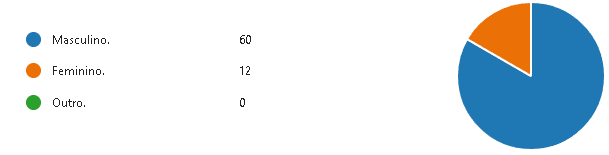
\includegraphics[scale=0.6]{figuras/1.png}
\caption{Questão 1}
\end{figure}

2. Qual disciplina você está cursando?

Nesta questão, sessenta e dois participantes responderam que estão cursando a disciplina de Requisitos de Software, enquanto apenas dez estão cursando a disciplina de Métodos de Desenvolvimento de Software.

\begin{figure}[H]
\centering
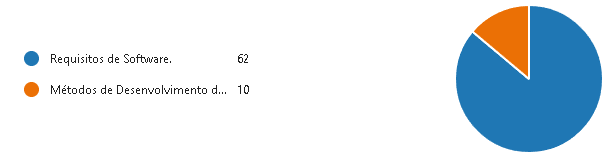
\includegraphics[scale=0.6]{figuras/2.png}
\caption{Questão 2}
\end{figure}

3. É sua primeira vez cursando a disciplina?

Dos setenta e dois participantes, sessenta e oito responderam que essa é a primeira vez que estão fazendo a mesma disciplina, enquanto apenas quatro estão refazendo a matéria.

\begin{figure}[H]
\centering
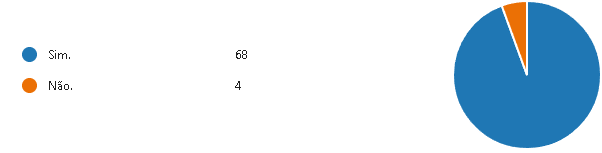
\includegraphics[scale=0.5]{figuras/3.png}
\caption{Questão 3}
\end{figure}

4. Você apresenta algum transtorno neurobiológico? (TDAH, TEA, distúrbios da aprendizagem, entre outros)

Nesta questão, nove participantes responderam que possuem algum tipo de transtorno neurobiológico, enquanto trinta e quatro responderam que não. Entretando, também possui uma parcela significativa de vinte e nove estudantes que não souberam responder sobre sua condição.

\begin{figure}[H]
\centering
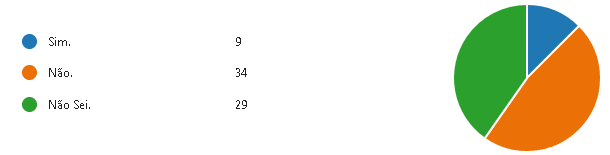
\includegraphics[scale=0.6]{figuras/4.png}
\caption{Questão 4}
\end{figure}

5. Menções (Exemplo: MM ou MS).

Referente ao retorno do feedback através apenas de menções, 56.9\% dos participantes votaram no valor 5, 29.4\% no valor 4, 11.1\% no valor 3, 1.4\% no valor 2 e 1.4\% no valor 1.

\begin{figure}[H]
\centering
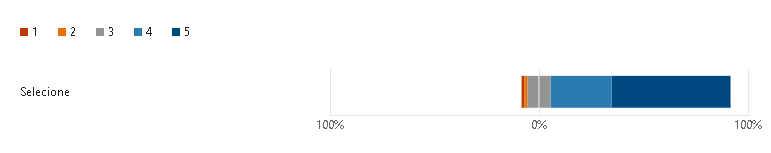
\includegraphics[scale=0.6]{figuras/5.png}
\caption{Questão 5}
\end{figure}

6. Visualizar o gabarito de cada questão.

Referente a visualização do gabarito de cada questão, 80.6\% dos participantes votaram no valor 5, 12.5\% no valor 4 e 6.9\% no valor 3, não existindo votos nos valores inferiores a 3, notando, assim, uma grande importância em saber qual é a resposta de determinada questão.

\begin{figure}[H]
\centering
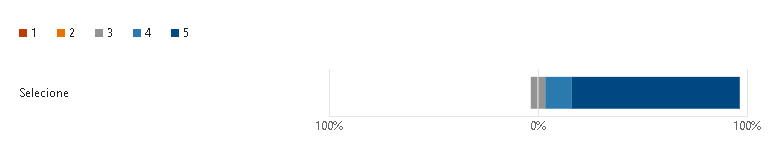
\includegraphics[scale=0.6]{figuras/6.png}
\caption{Questão 6}
\end{figure}

7. Exibir a explicação correspondente ao gabarito de cada questão.

Nesta questão, 75\% dos participantes votaram no valor 5, 16.7\% no valor 4, 6.9\% no valor 3 e 1.4\% no valor 2, não tendo respostas para o valor 1. Nota-se, então, um grande interesse na exibição de uma explicação para cada questão do questionário.

\begin{figure}[H]
\centering
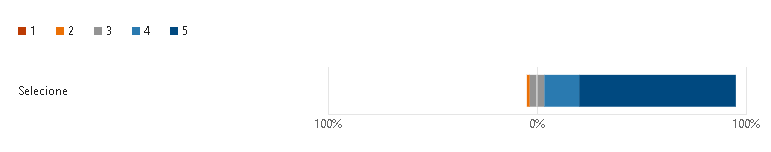
\includegraphics[scale=0.6]{figuras/7.png}
\caption{Questão 7}
\end{figure}


8. Indicação do material de estudo necessário para revisões do conteúdo.

Referente a indicação de material para estudo, 66.7\% dos participantes votaram no valor 5, 15.3\% no valor 4, 9.7\% no valor 3, 5.6\% no valor 2 e 2.8\% no valor 1. Com esses dados, é perceptivel o interesse por parte dos participantes na indicação de materias de estudo como complemento.

\begin{figure}[H]
\centering
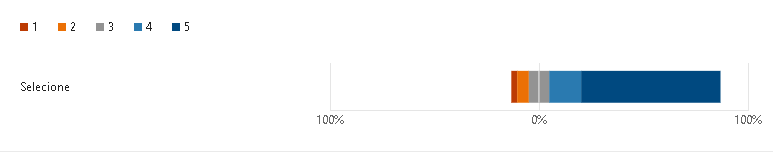
\includegraphics[scale=0.6]{figuras/8.png}
\caption{Questão 8}
\end{figure}

9. Visualizar os temas dos conteúdos que tiveram baixa taxa de acerto por meio de indicações textuais.

Referente a esta questão, 50\% dos participantes votaram no valor 5, 26.4\% no valor 4, 15.3\% no valor 3, 6.9\% no valor 2 e 1.4\% no valor 1.

\begin{figure}[H]
\centering
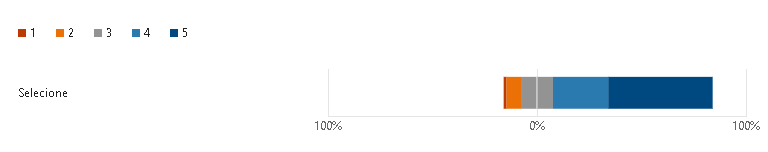
\includegraphics[scale=0.6]{figuras/9.png}
\caption{Questão 9}
\end{figure}

10. Visualizar um gráfico com uma divisão por temas em um conteúdo informando o desempenho na avaliação.

Quanto a este formato de feedback, 34.7\% dos participantes votaram no valor 5, 26.4\% no valor 4, 25\% no valor 3, 11.1\% no valor 2 e 2.8\% no valor 1. Nota-se que, comparado com as questões anteriores, não existe um grande interesse neste formato de feedback, podendo servir como feedback secundário.

\begin{figure}[H]
\centering
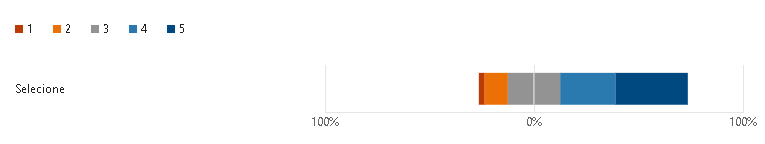
\includegraphics[scale=0.6]{figuras/10.png}
\caption{Questão 10}
\end{figure}

11. Reunião com o professor da disciplina para discutir sobre o resultado na avaliação e receber um Feedback humano.

Nesta questão, 22.2\% dos participantes votaram no valor 5, 19.4\% no valor 4, 43.1\% no valor 3, 8.3\% no valor 2 e 6.9\% no valor 1. Percebe-se um maior desinteresse por parte dos participantes neste formato de feedback, visto que mais de 50\% dos participantes votaram em um valor menor ou igual a três.

\begin{figure}[H]
\centering
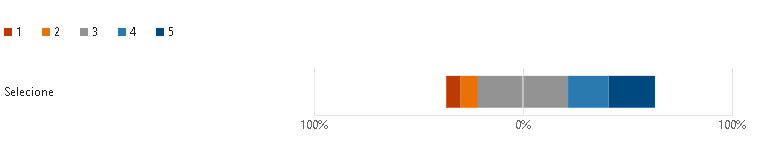
\includegraphics[scale=0.6]{figuras/11.png}
\caption{Questão 11}
\end{figure}

12. Relatório no formato PDF com um feedback descritivo do desempenho do aluno na avaliação. 

Para esta questão, 30.6\% dos participantes votaram no valor 5, 20.8\% no valor 4, 31.9\% no valor 3, 9.7\% no valor 2 e 6.9\% no valor 1. 

\begin{figure}[H]
\centering
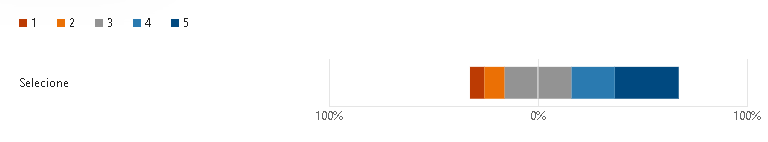
\includegraphics[scale=0.6]{figuras/12.png}
\caption{Questão 12}
\end{figure}

\chapter{Análise dos Resultados da Fase 1}

\section{Avaliação da confiabilidade}

Primeiramente, foi executado uma avaliação de confiabilidade para o formulário proposto. O método de avaliação utilizado foi o alfa de Cronbach. Para encontar o $\alpha$ foi utilizada a fórmula definida no capítulo de Metodologias.

O cálculo foi aplicado somente as questões de escala de classificação em que a escala de avaliação varia entre 1 e 5.

O cálculo do $\alpha$ de Cronbach gerou um valor exato de 0.753268, e este valor é classificado como "Alto", segundo os valores referenciados no capítulo de Metodologias. 

\section{Interpretação dos dados}

O mapa de calor a seguir, gerado pelo ChatGPT, representa as correlações entre diferentes formatos de feedback com base nas preferências dos alunos. Cada célula representa a correlação entre dois formatos de feedback, com valores variando de -1 a 1. Um valor de correlação próximo de 1 indica uma forte correlação positiva, significando que quando a preferência por um formato aumenta, a preferência pelo outro também tende a aumentar. Um valor próximo de -1 indicaria uma forte correlação negativa, o que não é observado neste conjunto de dados. Valores próximos de 0 indicam pouca ou nenhuma correlação.

\begin{figure}[H]
\centering
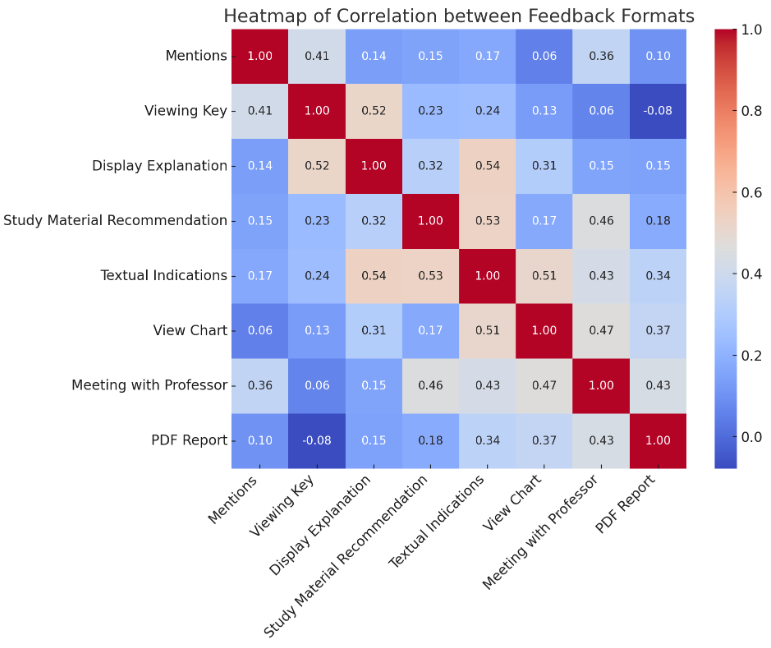
\includegraphics{figuras/heatmapfeedback.png}
\caption{Mapa de calor das correlações entre os formatos de feedback}
\end{figure}

A partir dos dados quantitativos, obtidos através do formulário, é possivel extrair diversas informações qualitativas relevantes, tais como: 

1. Explicação do gabarito de cada questão: Esse aspecto parece ser bastante valorizado, com muitos 5's, indicando que os respondentes veem grande importância em entender o porquê de suas respostas estarem certas ou erradas.

2. Indicação do material de estudo: Este item parece ter uma importância moderada a alta, com uma variação nas respostas, mas com muitos participantes ainda atribuindo a nota máxima.

3. Correlações mais fortes entre certos formatos, como explicação de gabarito e indicação de material de estudo, podem sugerir que os alunos veem esses métodos como complementares e eficazes em conjunto.

4. As respostas às questões visualizar gabarito de cada questão, explicação do gabarito, e indicação de material de estudo indicam uma preferência dos alunos por feedbacks que fornecem detalhes específicos e orientações claras. Isso sugere que os alunos valorizam feedbacks que não apenas apontam os erros, mas também orientam sobre como corrigi-los e melhorar.

5. As preferências mais baixas para temas com baixa taxa de acerto e gráfico de desempenho) podem indicar que, embora a visualização de dados seja útil, ela deve ser complementada com feedbacks mais explicativos e detalhados para ser eficaz.

6. As correlações observadas entre diferentes formatos de feedback sugerem que um sistema de IA para feedback formativo deve ser capaz de identificar padrões nos erros dos alunos e fornecer explicações detalhadas, juntamente com recursos e orientações para melhoria.

7. A IA poderia ser programada para reconhecer áreas problemáticas comuns entre os alunos e sugerir recursos específicos ou estratégias de estudo.

8. Visualizar Gabarito e Explicação do Gabarito: A alta preferência por esses formatos indica que os alunos valorizam não só saber as respostas corretas, mas também entender o raciocínio por trás delas. Isso sugere a importância de um sistema de IA que não se limite a apontar erros, mas forneça explicações claras e métodos para corrigi-los.

9. As correlações entre diferentes formatos de feedback apontam para a preferência dos alunos por um sistema holístico que integre múltiplos tipos de feedback. Por exemplo, a combinação de visualização de desempenho com explicações detalhadas pode ser particularmente eficaz.

10. Variação Mínima: As variações nas preferências de feedback com base no gênero são mínimas para a maioria dos formatos, indicando que ambos os gêneros têm preferências similares por esses tipos de feedback.

\begin{figure}[H]
\centering
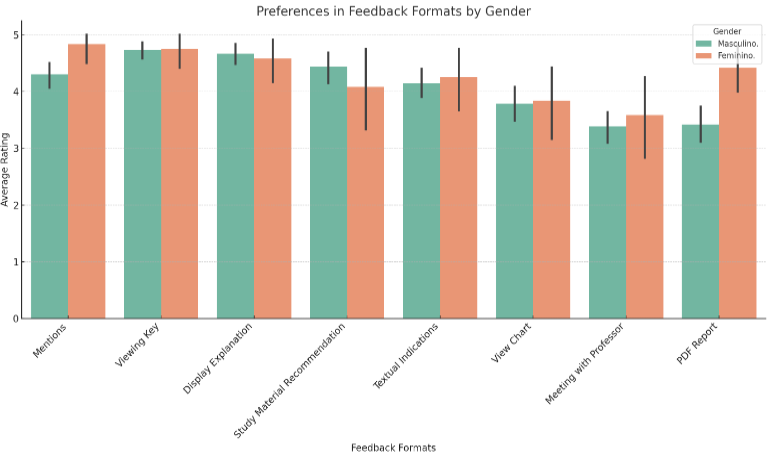
\includegraphics{figuras/gender_graph.png}
\caption{Gráfico representando a relação entre gênero e a avaliação do formato de feedback.}
\end{figure}

11. Algumas correlações entre diferentes formatos de feedback foram moderadamente altas, indicando que os alunos que preferem um tipo de feedback também tendem a preferir outros tipos similares. Por exemplo, a correlação entre Explicação do Gabarito e Indicação de Material de Estudo foi particularmente notável.

12. Foi observada correlações moderadas entre a presença de transtornos neurobiológicos e a preferência por certos tipos de feedback, como "Visualizar Gabarito" e "Reunião com o Professor". Essas correlações sugerem que alunos com transtornos neurobiológicos podem ter preferências específicas por feedbacks mais detalhados e interativos.

O gráfico a seguir, gerado pela ferramenta ChatGPT, mostra as correlações entre a presença de transtornos neurobiológicos nos respondentes e suas preferências por diferentes formatos de feedback:

\begin{figure}[!h]
\centering
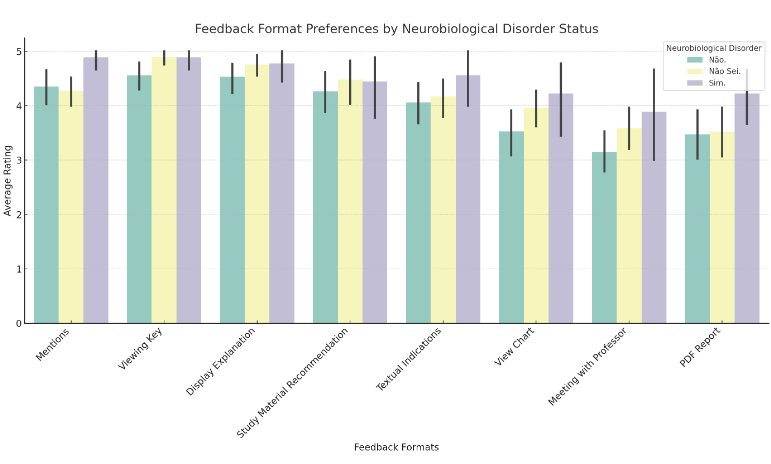
\includegraphics{figuras/neurological_graphic.png}
\caption{Correlações entre a presença de transtornos neurobiológicos nos respondentes e suas preferências por diferentes formatos de feedback}
\end{figure}

\begin{table}[H]
\centering
\begin{tabular}{|c|p{6cm}|p{8cm}|}
\hline
\textbf{Nº} & \textbf{Aspecto Analisado} & \textbf{Observações e Conclusões} \\
\hline
1 & Explicação do Gabarito de Cada Questão & Alta valorização com muitos 5's, indicando a importância de entender as respostas certas ou erradas. \\
\hline
2 & Indicação do Material de Estudo & Importância moderada a alta, com variação nas respostas. \\
\hline
3 & Correlação entre Explicação de Gabarito e Material de Estudo & Sugere que os alunos veem esses métodos como complementares. \\
\hline
4 & Preferência por Feedbacks Detalhados e Orientações Claras & Alunos valorizam feedbacks que orientam sobre como corrigir erros e melhorar. \\
\hline
5 & Preferências mais Baixas para Temas com Baixa Taxa de Acerto & Indica que feedbacks devem ser complementados com detalhes explicativos. \\
\hline
6 & Correlações entre Formatos de Feedback & Sistema de IA deve identificar padrões nos erros e fornecer explicações detalhadas e recursos para melhoria. \\
\hline
7 & IA para Reconhecimento de Áreas Problemáticas & Sugerir recursos específicos ou estratégias de estudo. \\
\hline
8 & Visualizar Gabarito e Explicação do Gabarito & Alta preferência indica a valorização do entendimento do raciocínio por trás das respostas. \\
\hline
9 & Correlações entre Diferentes Formatos de Feedback & Preferência por um sistema holístico que integre múltiplos tipos de feedback. \\
\hline
10 & Variação Mínima com Base no Gênero & Preferências similares entre os gêneros para a maioria dos formatos de feedback. \\
\hline
11 & Correlações entre Diferentes Tipos de Feedback & Alunos que preferem um tipo de feedback tendem a preferir outros similares. \\
\hline
12 & Correlações e Transtornos Neurobiológicos & Alunos com transtornos neurobiológicos podem preferir feedbacks mais detalhados e interativos. \\
\hline
\end{tabular}
\caption{Resumo das Análises dos Dados Quantitativos do Formulário}
\end{table}


\section{Discussão}

A partir dos dados apresentados, os três formatos de feedback com maior dominância de importância foram: "Visualizar o gabarito de cada questão", "Exibir a explicação correspondente ao gabarito de cada questão" e "Indicação do material de estudo necessário para revisões do conteúdo". Estes três formatos corroboram com a ideia de feedback formativo, que, segundo Shute \cite{shute2008focus}, é definido como a informação comunicada ao aluno que pretende modificar seu pensamento ou comportamento com o propósito de melhorar o aprendizado, ou seja, consiste em toda informação que permite ao aluno identificar o que falta fazer e como fazer para alcançar o esperado.

Também é importante considerar as limitações deste estudo. Primeiramente, a amostra foi limitada a alunos de duas disciplinas específicas, o que pode restringir a generalização dos resultados para outros contextos educacionais ou disciplinas. Além disso, o estudo focou principalmente em correlações entre preferências de feedback e certos fatores demográficos, como gênero e a presença de transtornos neurobiológicos, mas não explorou outras variáveis importantes que podem influenciar as preferências de feedback, como o contexto cultural, o histórico educacional prévio ou o estilo de aprendizagem individual.
\chapter{Análise de Viabilidade Técnica}

\section{Introdução}

Neste capítulo, discutiremos a viabilidade técnica do desenvolvimento de uma Inteligência Artificial para aprimorar a avaliação individual nas disciplinas de requisitos de software e métodos de desenvolvimento de software na Universidade de Brasília. Exploraremos as tecnologias e ferramentas necessárias para analisar o desempenho dos alunos, e fornecer \textit{feedbacks} formativos.

\section{Objetivos Técnicos}

Os objetivos técnicos deste trabalho refletem em analisar o desempenho dos alunos em avaliações individuais das disciplinas requisitos de software e métodos de desenvolvimento de software, para gerar \textit{feedbacks} formativos por meio de uma inteligência artificial.

Existindo uma comunicação externa à plataforma utilizada nas disciplinas, o Microsoft Forms, sendo executada por meio de uma automação com a ferramenta Microsoft Power Automate, que provê a comunicação entre os dados das avaliações individuais dos alunos e os \textit{feedbacks} formativos gerados pela inteligência artificial.

\section{Requisitos da Ferramenta}

A implementação para alcançar o objetivo técnico desejado pode exigir o uso de diversas ferramentas de inteligência artificial e \textit{frameworks}. Algumas considerações incluem:

\begin{itemize}
  \item Processamento de Linguagem Natural (PLN): para que, após a compreensão e análise de desempenho, possamos gerar \textit{feedback} textual de forma coerente e compreensível.
  \item Integração com API Externa: considerando a possibilidade de enviar dados para uma API externa que receberá os resultados das avaliações individuais dos estudantes e retornará o \textit{feedback} gerado pela IA.
\end{itemize}

\section{Tecnologias Idealizadas}

Levando em consideração os requisitos da ferramenta a ser construída, foi planejada a utilização das seguintes tecnologias em cada ambiente:

\begin{itemize}
  \item PLN: biblioteca NLTK (\textit{Natural Language Toolkit}), SpaCy, modelos de linguagem pré-treinados como BERT e ferramentas da OpenAI, como o modelo GPT (\textit{Generative Pre-trained Transformer}).
  \item API Externa: utilizar o \textit{framework} FastAPI, para desenvolver uma API em Python que se comunique com o modelo de inteligência artificial.
\end{itemize}

Além disso, será desenvolvido um fluxo de trabalho que integra o Microsoft Forms e a API externa. Os dados das avaliações individuais realizadas pelos discentes serão enviados automaticamente para a API por meio do Microsoft Power Automate. Após o processamento das informações, o \textit{feedback} formativo gerado será disponibilizado para os alunos em um arquivo no formato PDF, acessível diretamente através da plataforma de e-mail.

\section{Resultados da Análise de Viabilidade Técnica}

Após a análise de viabilidade técnica, foi constatado que a integração de uma Inteligência Artificial (IA) para aprimorar a avaliação individual nas disciplinas de requisitos de software e métodos de desenvolvimento de software é tecnicamente viável. A análise considerou o uso de um modelo de Processamento de Linguagem Natural (PLN) para a geração de \textit{feedbacks} textuais personalizados, a integração com APIs externas para facilitar o fluxo de dados e a utilização de tecnologias como FastAPI e ferramentas da OpenAI.

A integração proposta entre Microsoft Forms, Microsoft Power Automate, e a API desenvolvida com FastAPI foi avaliada como uma solução robusta para automatizar o processo de envio e recepção de dados das avaliações individuais.

Em resumo, a análise de viabilidade técnica validou a proposta inicial, demonstrando que as tecnologias idealizadas são capazes de suportar o desenvolvimento da ferramenta pretendida, proporcionando melhorias significativas no processo de avaliação e no fornecimento de \textit{feedbacks} formativos aos alunos.
\chapter{Planejamento}

\section{Trabalho de Conclusão de Curso 1}

Para o planejamento do TCC1, as atividades levantadas serão descritas na tabela a seguir, para facilitar no entendimento, as siglas levarão em consideração a ordem cronológica do desenvolvimento de cada atividade:

\begin{table}[!ht]
\centering
\begin{tabularx}{\textwidth}{|X|X|}
\hline
\textbf{Sigla} & \textbf{Descrição} \\
\hline
A1 & Criar estrutura do relatório do TCC1 no Overleaf \\ \hline
A2 & Criar planejamento  \\\hline
A3 & Desenvolver o Resumo \\\hline
A4 & Estudar documentação técnica do Moodle \\\hline
A5 & Desenvolver o capítulo 1 \\\hline
A6 & Desenvolver o capítulo 2 \\\hline
A7 & Criar formulário de pesquisa sobre tipos de feedbacks \\\hline
A8 & Desenvolver o capítulo 3 \\\hline
A9 & Criar roteiro para entrevista em grupo focal \\\hline
A10 & Encontrar participantes para entrevista em grupo focal \\\hline
A11 & Realizar entrevista em grupo focal \\\hline
A12 & Adaptar formulário de pesquisa com dados coletados na entrevista em grupo focal \\\hline
A13 & Divulgar formulário de pesquisa para as disciplinas REQ e MDS \\\hline
A14 & Desenvolver o capítulo 4 \\\hline
A15 & Desenvolver o capítulo 5 \\\hline
A16 & Pesquisar tecnologias para viabilizar a ferramenta \\\hline
A17 & Desenvolver o capítulo 6 \\\hline
A18 & Desenvolver o capítulo 7 \\\hline
A19 & Desenvolver o capítulo 8 \\\hline
A20 & Corrigir relatório baseando-se na revisão do orientador \\\hline
A21 & Preparar apresentação do TCC1 para a banca avaliadora \\\hline
A22 & Apresentar o TCC1 para a banca avaliadora \\\hline
A23 & Realizar retrospectiva sobre o TCC1 \\\hline
\end{tabularx}
\caption{Tabela de siglas de atividades do TCC1}
\end{table}

\pagebreak

A tabela a seguir ligará as atividades com os seus respectivos períodos:

\pagebreak

\begin{table}[!ht]
\centering
\begin{tabularx}{\textwidth}{|X|X|}
\hline
\textbf{Período} & \textbf{Atividade} \\
\hline
05/09/2023 - 12/09/2023 & A1, A2 \\ \hline
13/09/2023 - 19/09/2023 & A2, A3 \\ \hline
20/09/2023 - 26/09/2023 & A3, A4, A5 \\ \hline
27/09/2023 - 03/10/2023 & A4, A5, A6 \\ \hline
04/10/2023 - 10/10/2023 & A4, A6, A7 \\ \hline
11/10/2023 - 17/10/2023 & A7, A8 \\ \hline
18/10/2023 - 24/10/2023 & A7, A8 \\ \hline
25/10/2023 - 31/10/2023 & A8, A9, A10, A11 \\ \hline
01/11/2023 - 07/11/2023 & A12, A13 \\ \hline
08/11/2023 - 14/11/2023 & A14, A15 \\ \hline
15/11/2023 - 21/11/2023 & A16, A17, A18, A19 \\ \hline
22/11/2023 - 28/11/2023 & A20 \\ \hline
29/11/2023 - 05/12/2023 & A20 \\ \hline
06/12/2023 - 12/12/2023 & A21 \\ \hline
13/12/2023 - 19/12/2023 & A22 \\ \hline
20/12/2023 - 23/12/2023 & A23 \\ \hline
\end{tabularx}
\caption{Tabela de atividades por período do TCC1}
\end{table}

\section{Trabalho de Conclusão de Curso 2}

Para o planejamento do TCC2, as atividades levantadas serão descritas na tabela a seguir, para facilitar no entendimento, as siglas levarão em consideração a ordem cronológica do desenvolvimento de cada atividade:

\begin{table}[!ht]
\centering
\begin{tabularx}{\textwidth}{|X|X|}
\hline
\textbf{Sigla} & \textbf{Descrição} \\
\hline
A1 & Pesquisar e desenvolver prova de conceito \\ \hline
A2 & Estudar a conexão da API com a plataforma Microsoft Forms e Automate \\\hline
A3 & Desenvolver a API \\\hline
A4 & Desenvolvimento a ferramenta de IA \\\hline
A5 & Documentar o desenvolvimento \\\hline
A6 & Testar a API \\\hline
A7 & Testar a ferramenta de IA \\\hline
A8 & Conectar a API ao Microsoft Automate \\\hline
A9 & Testar a conexão da API com o Microsoft Automate e a ferramenta de IA \\\hline
A10 & Realizar teste em produção nas disciplinas MDS e REQ \\\hline
A11 & Corrigir qualquer erro que existir na ferramenta \\\hline
A12 & Corrigir o trabalho baseando-se na revisão do orientador \\\hline
A13 & Preparar apresentação do TCC2 para a banca avaliadora \\\hline
A14 & Apresentar o TCC2 para a banca avaliadora \\\hline
\end{tabularx}
\caption{Tabela de siglas de atividades do TCC2}
\end{table}

\pagebreak

A tabela a seguir ligará as atividades com os seus respectivos períodos:

\begin{table}[!ht]
\centering
\begin{tabularx}{\textwidth}{|X|X|}
\hline
\textbf{Período} & \textbf{Atividade} \\
\hline
01/01/2024 - 14/01/2024 & A1, A2, A5 \\ \hline
15/01/2024 - 28/01/2024 & A1, A2, A5 \\ \hline
29/01/2024 - 11/02/2024 & A1, A2, A5 \\ \hline
12/02/2024 - 25/02/2024 & A1, A2, A5 \\ \hline
26/02/2024 - 10/03/2024 & A3, A4, A5 \\ \hline
11/03/2024 - 24/03/2024 & A3, A4, A5 \\ \hline
25/03/2024 - 07/04/2024 & A4, A5, A6  \\ \hline
08/04/2024 - 21/04/2024 & A4, A5, A6, A8 \\ \hline
22/04/2024 - 05/05/2024 & A5, A7, A8 \\ \hline
06/05/2024 - 19/05/2024 & A5, A9 \\ \hline
20/05/2024 - 02/06/2024 & A10 \\ \hline
03/06/2024 - 16/06/2024 & A10, A11 \\ \hline
17/06/2024 - 30/06/2024 & A10, A12, A13 \\ \hline
01/07/2024 - 15/07/2024 & A10, A14 \\ \hline
\end{tabularx}
\caption{Tabela de atividades por período do TCC2}
\end{table}


\chapter{Conclusão/Considerações Finais}

\section{Resumo das Descobertas}

Este estudo buscou aprimorar o processo de avaliação acadêmica na Universidade de Brasília, com foco nas disciplinas de requisitos de software e métodos de desenvolvimento de software. As principais descobertas incluem a necessidade de feedbacks formativos detalhados e personalizados, em vez de simples avaliações numéricas. Utilizando ferramentas de Inteligência Artificial (IA) para a análise de dados, o estudo revelou que os alunos preferem feedbacks que oferecem explicações detalhadas, indicações de material de estudo e visualização clara dos gabaritos. A confiabilidade desses achados foi validada pelo coeficiente alfa de Cronbach, que obteve uma classificação alta. Adicionalmente, a análise da viabilidade técnica confirmou a possibilidade de implementar a solução de IA proposta, usando tecnologias como PLN e integração com APIs externas.

\section{Implicações}

As implicações destas descobertas são significativas para o campo da educação em ciências da computação. Ao enfatizar a importância de feedbacks formativos ricos em informações, este estudo sugere uma mudança de paradigma nas práticas avaliativas, movendo-se de uma abordagem quantitativa para uma mais qualitativa e enriquecedora. Essa mudança pode levar a um melhor engajamento dos alunos, facilitando uma compreensão mais profunda do conteúdo e incentivando a autorreflexão. Além disso, a implementação de soluções baseadas em IA na avaliação acadêmica levanta considerações importantes sobre a privacidade dos dados dos alunos e a necessidade de alinhamento ético nas práticas educacionais.

\section{Trabalhos futuros}

No desenvolvimento subsequente, especificamente para o Trabalho de Conclusão de Curso 2, a atenção será voltada para a implementação técnica de uma solução de Inteligência Artificial que ofereça feedbacks formativos detalhados e personalizados, mais especificamente, é proposto, para o TCC 2, que os formatos de feedbacks a serem trabalhados sejam "Exibir a explicação correspondente ao gabarito de cada questão" e "Visualizar os temas dos conteúdos que tiveram baixa taxa de acerto por meio de indicações textuais". Como foi descrito no capítulo 6, este próximo passo envolverá a construção e integração de um sistema de IA, com a plataforma do Moodle, que analise as avaliações dos alunos com eficiência e gere feedbacks formativos, mergulhando mais profundamente em tecnologias de Processamento de Linguagem Natural (PLN) e utilizando modelos avançados de linguagem.

A fase seguinte abrangerá testes abrangentes do sistema para validar sua eficácia. Esses testes irão verificar a precisão do feedback gerado, a usabilidade da interface e a integração com a plataforma de aprendizado existente. Paralelamente, será conduzido um estudo piloto em contextos reais de aprendizado, utilizando a solução de IA para coletar dados sobre a receptividade dos alunos, a eficácia do feedback e o impacto na aprendizagem e no engajamento dos estudantes.

Após a coleta desses dados, uma análise detalhada será realizada para entender a eficácia do sistema e identificar áreas para melhorias. Ajustes no sistema de IA poderão ser feitos com base no feedback dos usuários e na análise de desempenho. Além disso, será dada atenção especial à personalização e customização dos feedbacks, a fim de atender às necessidades individuais dos alunos, considerando diferentes estilos de aprendizagem e níveis de compreensão.

Também será essencial explorar as implicações éticas e de privacidade relacionadas ao uso de IA na educação, garantindo que a solução seja não apenas eficiente, mas também segura e ética. Por fim, a possibilidade de expandir a aplicação da solução de IA para outras disciplinas e contextos educacionais será avaliada, explorando sua adaptabilidade e eficácia em diferentes áreas de estudo.

Portanto, o TCC2 visa não apenas desenvolver uma solução tecnológica para feedbacks formativos, mas também contribuir significativamente para o campo da educação tecnológica, melhorando a experiência de aprendizado dos alunos e fornecendo insights valiosos para futuras inovações educacionais.

\section{Conclusão}

Em conclusão, este estudo ressalta a importância do feedback formativo no contexto educacional, demonstrando que a inclusão de feedback detalhado e personalizado, apoiado por tecnologias de IA, pode significativamente enriquecer a experiência de aprendizagem dos alunos. As descobertas deste trabalho servem como um ponto de partida para pesquisas futuras e para o desenvolvimento de práticas avaliativas mais eficazes e inclusivas na educação superior.

\bookmarksetup{startatroot} 

\postextual

\bibliography{bibliografia} 
\printindex

\end{document}

